\chapter{Links to other computing codes}

This chapter provides information on interoperability of \MCS with
other codes, and provide links to other sources of information on this topic.

\section{\MCS and MANTID}
As of \MCS 2.1 and MANTID 3.2, the teams of the two codes provide a mechanism to transfer simulated \MCS
events and monitor data to MANTID, via NeXus files.

\subsection{System requirements}
To enable the software link, you need the following codes installed on
your system:
\begin{itemize}
\item{\MCS 2.1 or newer}
\item{NeXus libraries from \verb+http://nexusformat.org+ \footnote{For Mac OS X you may get
    better milage via the Mantid github site}}
\item{Mantid 3.2 or newer}
\item{On Mac OS X 10.8 and newer you may need to install one of the
    below compilers, as the default clang on OS X causes problems for
    the link, especially when used together with MPI}
  \begin{itemize}
  \item{Intel C}
  \item{gcc from \verb+http://hpc.sourceforge.net+}
  \end{itemize}
\end{itemize}

\subsection{Requirements for the instrument file}
A special naming convention in the instrument file is needed for the
automatic transfer of geometry to a Mantid IDF file:

\begin{itemize}
\item The location of the source must be indicated by a component
  named sourceMantid. Note that in the case of a curved instrument
  geometry, you should probably add an Arm where Mantid 'expects' the
  source to be, i.e.: defining a location displaced the correct
  source-sample distance, parallel to the incoming beam direction at
  the sample.
\item The location of the sample must be indicated by a component
  named sampleMantid
\item One or more Monitor\_nD components need to be added in either
  rectangular- or cylindrical geometry and with a set of special
  flags, as shown below
\item Rectangular monitor
  \begin{mcstas}
    COMPONENT nD_Mantid_0 = Monitor_nD(
    options ="mantid square x limits=[-0.2 0.2] bins=128 y limits=[-0.2 0.2] bins=128, neutron pixel t, list all neutrons",
    xmin = -0.2,
    xmax = 0.2,
    ymin = -0.2,
    ymax = 0.2,
    restore_neutron = 1,
    filename = "bank01_events.dat")
  AT (0, 0, 3.2) RELATIVE sampleMantid 
\end{mcstas}
\item Cylindrical monitor
  \begin{mcstas}
    COMPONENT nD_Mantid_01 = Monitor_nD(xwidth=(4.0-0.0005-0.00002)*2, yheight=3,
    options="mantid banana, theta limits=[-73.36735 73.36765] bins=100, y limits=[-1.5 1.5] bins=300, neutron pixel t, list all neutrons", restore_neutron=1)
    AT (0,0,0) RELATIVE center_det
\end{mcstas}
\end{itemize}
The two instruments \verb+templateSANS_Mantid.instr+ and
\verb+ILL_H16_IN5_Mantid.instr+ have these features enabled.

Other, ordinary \MCS monitors will also be visible in the resulting
Mantid workspace, but will not be easily processible using the Mantid
TOF data reduction schemes.

\subsection{Compiling and running your simulation for Mantid output}
Geometry information in Mantid is handled via a so-called Instrument
Definition File (IDF) in xml-format, possibly embedded in a NeXus
file. The creation of the IDF and related NeXus file is handled in the
following steps:
\begin{enumerate}
\item First of all, enable NeXus in the compilation process:
 \begin{mcstas} 
   export MCSTAS_CFLAGS="-g -lm -O2 -DUSE_NEXUS -lNeXus"
 \end{mcstas}
\item Compile the instrument via the mcrun utility (add \verb+--mpi+
  if you need parallelization support):
 \begin{mcstas} 
   mcrun -c ILL_H16_IN5_Mantid.instr -n0
 \end{mcstas}
\item Generate the IDF via the mcdisplay utility (and press enter
  until the simulation runs):
 \begin{mcstas} 
   mcdisplay --format=Mantid ILL_H16_IN5_Mantid.instr -n0
 \end{mcstas}
\item Finally, run a simulation with NeXus output:
 \begin{mcstas} 
   mcrun --format=NeXus ILL_H16_IN5_Mantid.instr 
 \end{mcstas} 
\end{enumerate}


\subsection{Looking at instrument output in Mantid}
In Mantid, your new NeXus file should behave more or less as usual,
that is
\begin{itemize}
\item Start by loading the file using either the Load button or the
algorithm LoadMcStas to load the event file. 
\item After a succesful load, you should have a workspace group with
this content
\begin{center}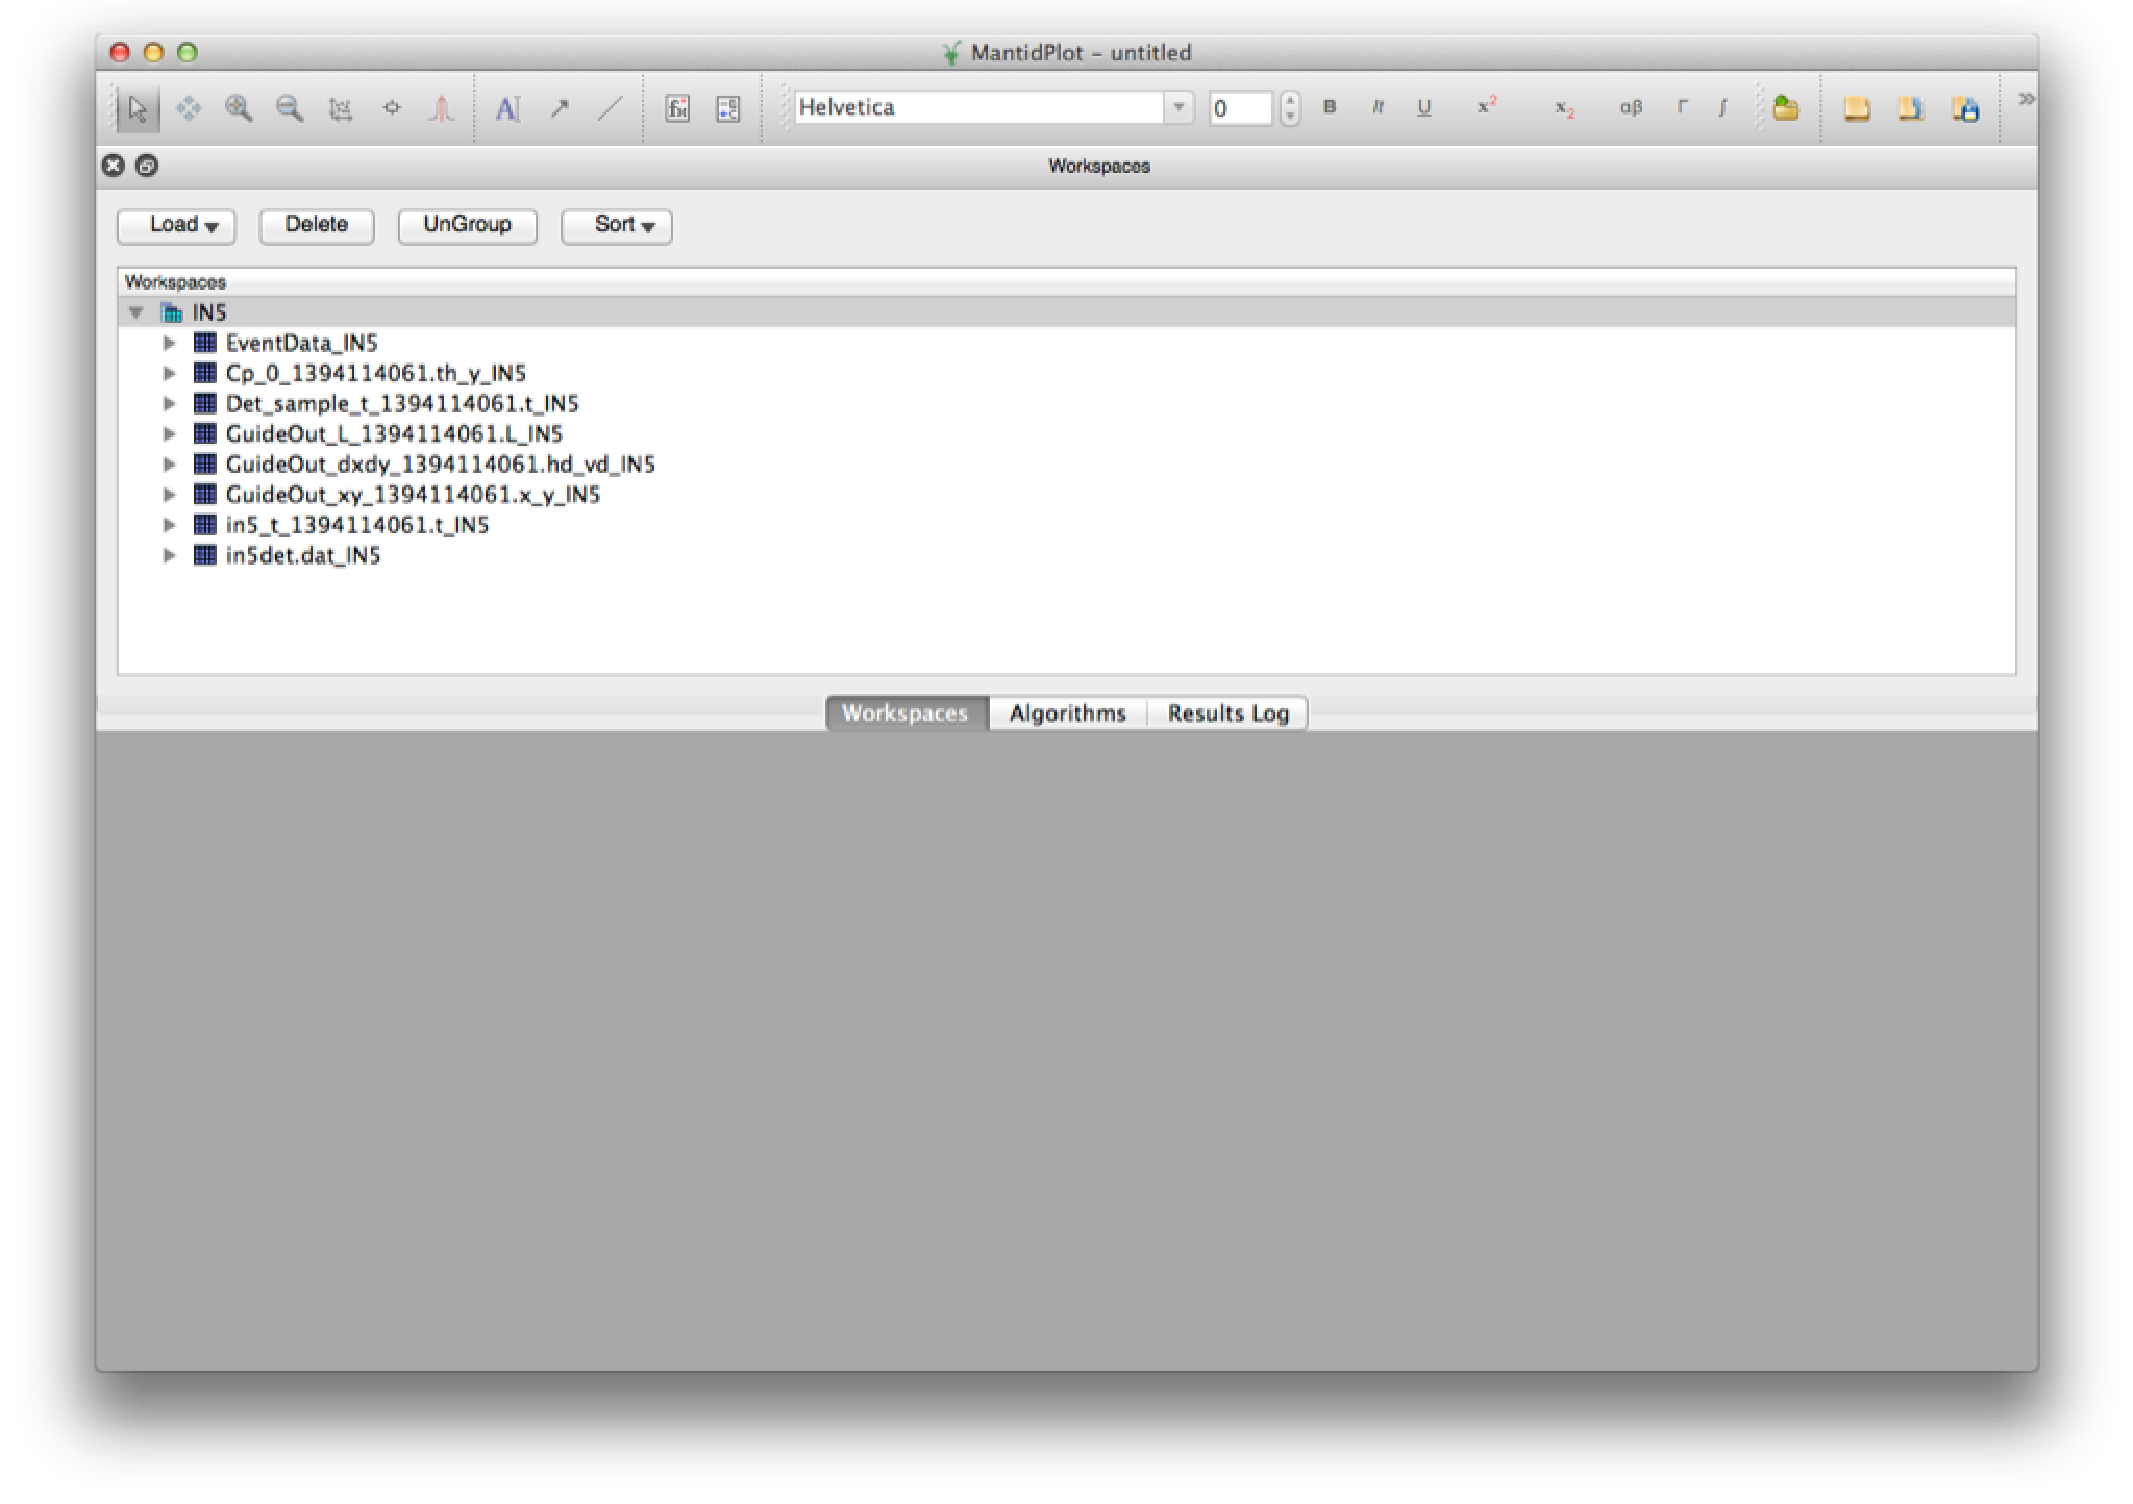
\includegraphics[width=.5\textwidth]{figures/mantid-1}\end{center}
\item Plot the histogram event data stored in the monitor Cp\_0...\\
\begin{center}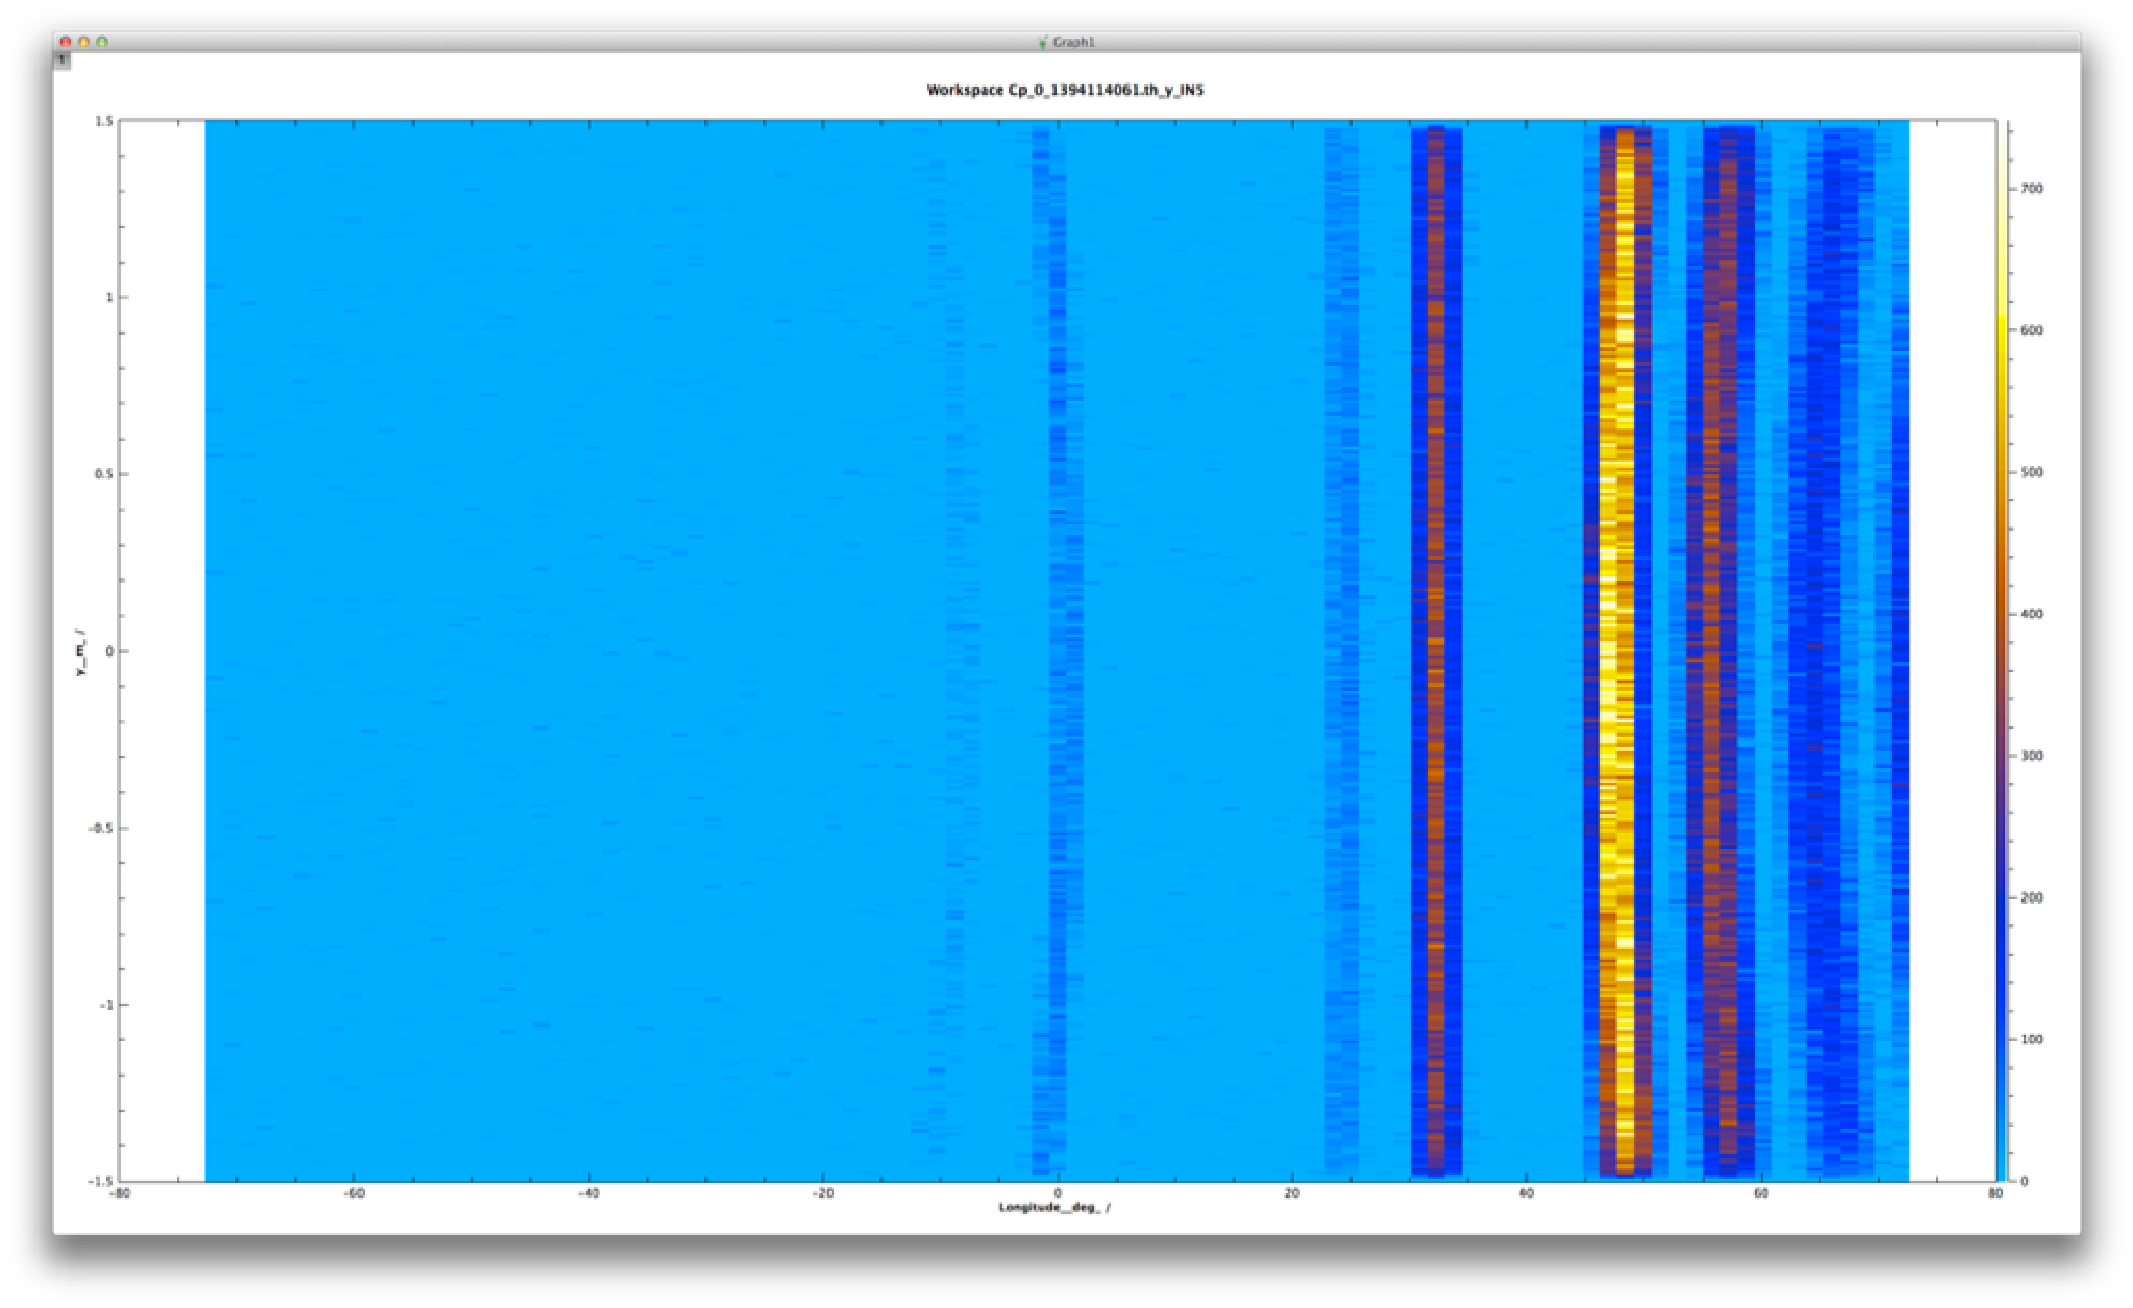
\includegraphics[width=.5\textwidth]{figures/mantid-2}\end{center}
\item Plot the TOF events on the full instrument geometry. In this
step a bit of zooming and translation may be needed to show a nice
view of the instrument.
\begin{center}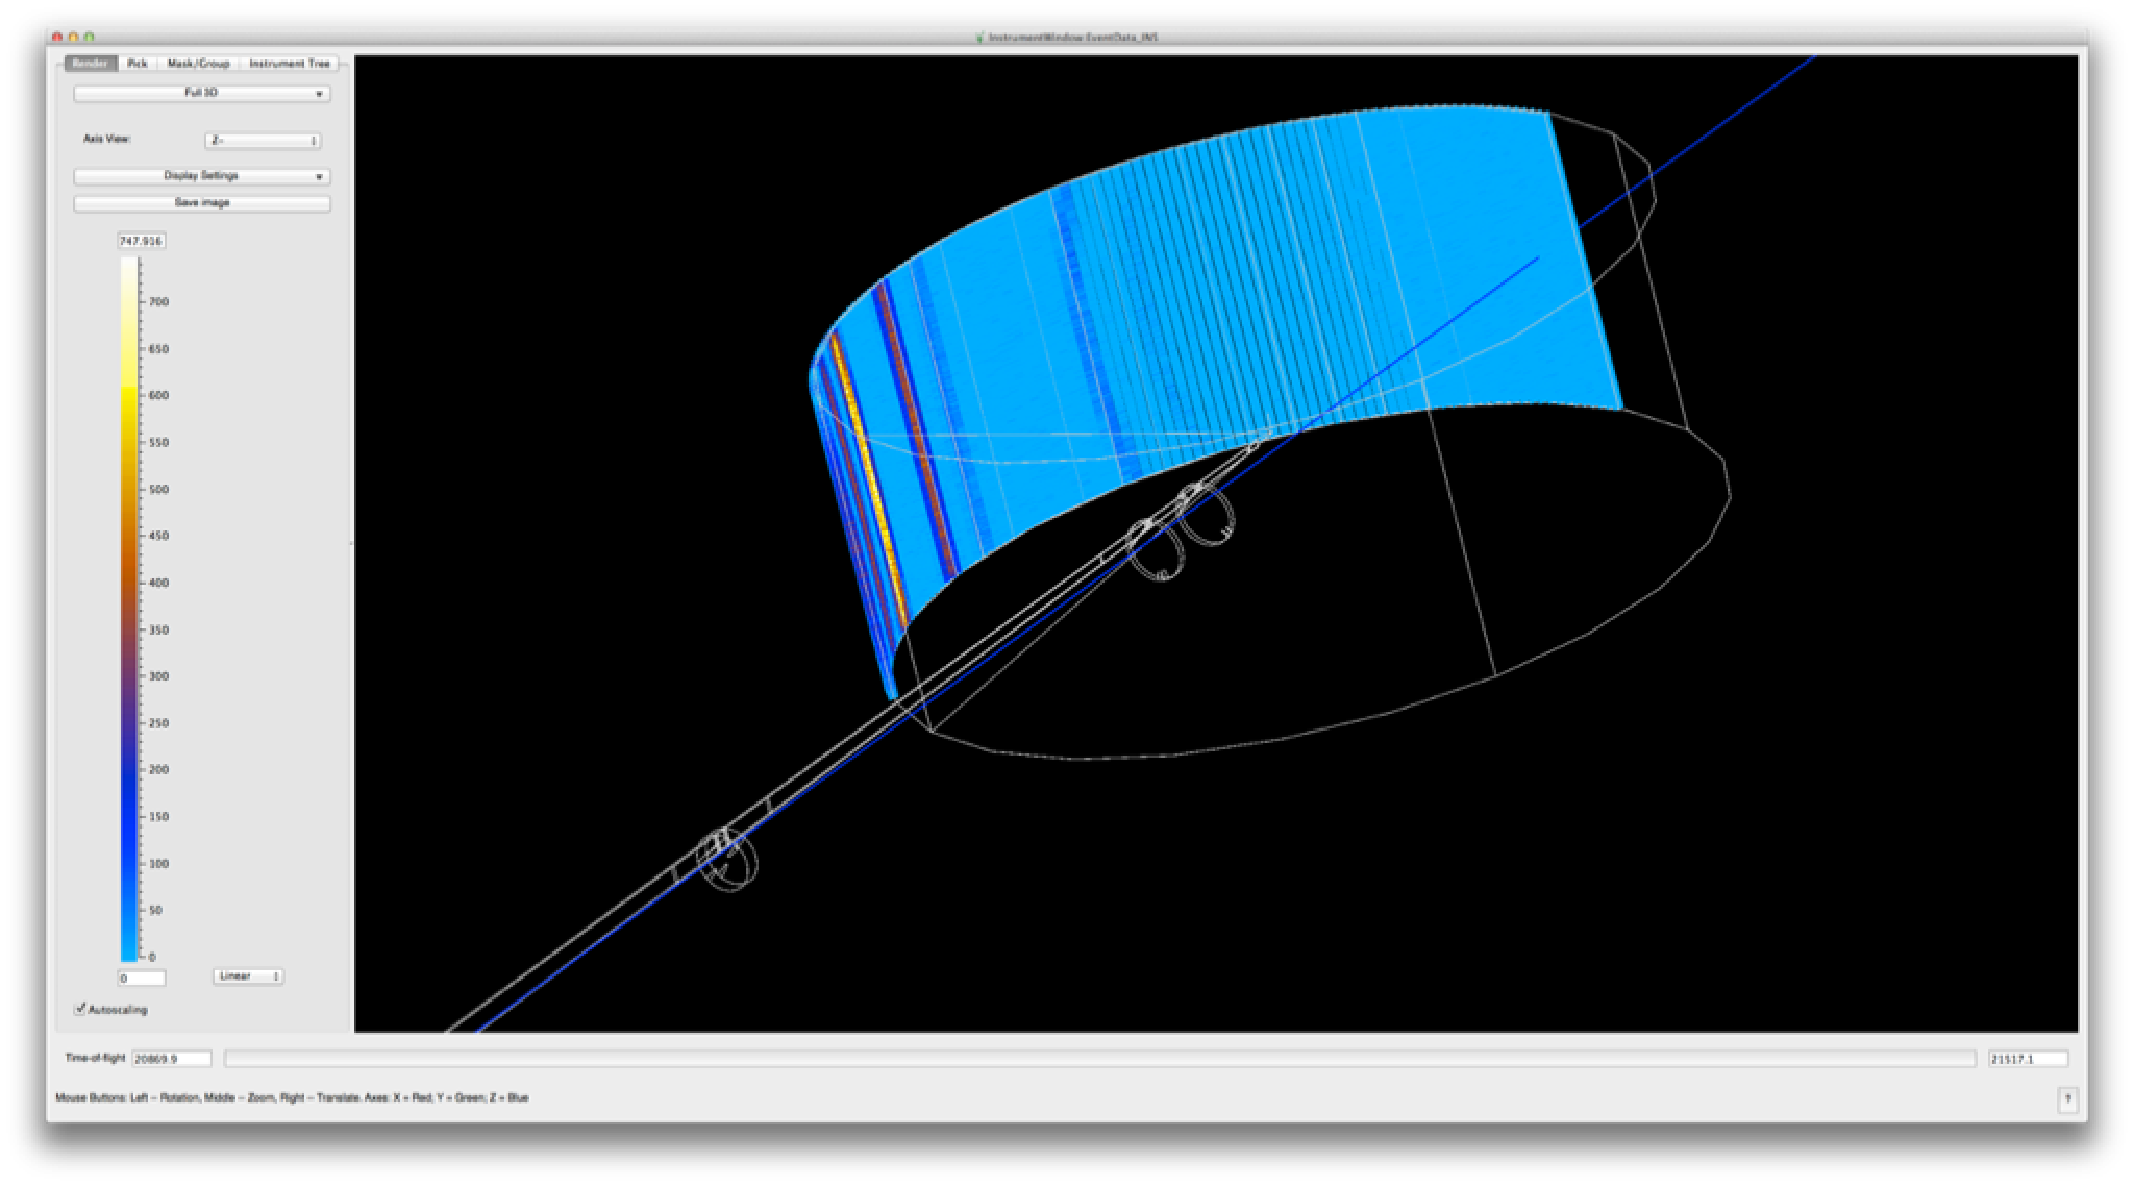
\includegraphics[width=.5\textwidth]{figures/mantid-3}\end{center}
\end{itemize}
The instrument \verb+ILL_H16_IN5_Mantid.instr+ included in \MCS 2.1 will load and present
simulated event-data, but the current time-definition of the event data does not comply
fully with Mantid for data-reduction purposes - this should be
corrected for the next \MCS release.

\section{\MCS and MCNP(X)}

